\chapter{Product}\label{chap:product}

\section{Implementation of the prototype}

\section{Programming language choice}

% TODO: Table of languages

\subsection{Functional programming paradigms}

% PHP vs Clojure

\subsection{Web programming with functional languages}

% Similarities to JavaScript (and it's popularity)

\section{Prototype rewrite in LISP}

\section{Persistent storage}
\subsection{Yet Another Protein Schema}

%%%%%%%%%%%%%%%%%%%%%%%%%%%
%% Listing: yaps-example %%
%%%%%%%%%%%%%%%%%%%%%%%%%%%
\lstset{language=JavaScript}
\begin{lstlisting}[label=lst:yaps-example,caption={
      [Example YAPS encoded dataset]
      An example YAPS encoded dataset, containing a single record.}]
{
  "Encoding": "yaps",
  "Version": 4,
  "Date": "2014-04-20 02:29:48",
  "Author": "chris@vm-ubuntu",
  "Agent": "/home/chris/src/pip-db/tools/csv2yaps/csv2yaps.js",
  "Source": "/home/chris/dataset-test.txt",
  "No-Of-Records": 1,
  "Records": [
    {
      "Protein-Names": [
        "Acetoacetyl-CoA thiolase",
        "Acetyl-CoA acetyltransferase"
      ],
      "EC": "2.3.1.9",
      "Source": "Saccharomyces cerevisiae (Yeast)",
      "Location": "Cytosol",
      "MW-Min": "140000",
      "MW-Max": "140000",
      "No-Of-Iso-Enzymes": "1",
      "pI-Min": "5.3",
      "pI-Max": "5.3",
      "Temperature-Min": "4",
      "Temperature-Max": "4",
      "Method": "Isoelectric focusing",
      "Full-Text": "http://www.jbc.org/content/246/14/4424 ...",
      "PubMed": "http://www.ncbi.nlm.nih.gov/pubmed/557183 ...",
      "Species-Taxonomy": "http://www.ncbi.nlm.nih.gov/Tax ...",
      "Protein-Sequence": "http://www.uniprot.org/uniprot/ ...",
      "Sequence-Name": ">sp|P41338|THIL_YEAST Acetyl-CoA a ..."
      "Sequence-Data": "MSQNVYIVSTARTPIGSFQGSLSSKTAVELGAVA ..."
    }
}
\end{lstlisting}

\section{Search engine design}

%%%%%%%%%%%%%%%%%%%%%%%%%%%%%
%% Table: query-components %%
%%%%%%%%%%%%%%%%%%%%%%%%%%%%%
\begin{table}[H]
\centering
\begin{tabular}{| c | c | l |}
\hline
\textbf{Family} & \textbf{Symbol} & \textbf{Definition}\\
\hline
& $id$ & Unique identifier\\
$N$ & $q_0 \ldots q_n$ & Any keywords\\
$N$ & $a_0 \ldots a_n$ & All keywords\\
$N$ & $n_0 \ldots n_n$ & Not keywords\\
$N$ & $eq$ & Exact phrase\\
$P$ & $p_l$, $p_h$ & Minimum and maximum isoelectric point\\
$P$ & $m_l$, $m_h$ & Minimum and maximum molecular weight\\
$P$ & $e_0$, $e_1$, $e_2$, $e_3$ & Enzyme commission number\\
$P$ & $l_s$ & Source location\\
$P$ & $l_l$ & Organ or sub-cellular location\\
$P$ & $f_n$ & FASTA sequence name\\
$P$ & $f_s$ & FASTA sequence string\\
$E$ & $m$ & Experimental method\\
$E$ & $t_l$, $t_h$ & Minimum and maximum experimental temperature\\
\hline
\end{tabular}
\caption[Query component symbols and their definitions]{Query component symbols and their definitions.}
\label{tab:query-components}
\end{table}


% TODO: example searches (and URLs) from appendix

\newpage

%%%%%%%%%%%%%%%%%%%%%%%%
%% Figure: query-tree %%
%%%%%%%%%%%%%%%%%%%%%%%%
\begin{figure}[t]
\centering
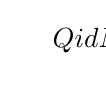
\begin{tikzpicture}
\tikzset{level distance=50pt, sibling distance=1.5pt}
  \Tree [.{$Q$}
    [.{$id$} ]
    [.{$N$}
      [.{$Q$}
        [. \node(q0){$q_0$}; ]
        [. \node(qn){$q_n$}; ]
      ]
      [.{$A$}
        [. \node(a0){$a_0$}; ]
        [. \node(an){$a_n$}; ]
      ]
      [. {$N$}
        [. \node(n0){$n_0$}; ]
        [. \node(nn){$n_n$}; ]
      ]
      [.{$eq$} ]
    ]
    [.{$P$}
      [.{$P$}
        [.{$p_l$} ]
        [.{$p_h$} ]
      ]
      [.{$M$}
        [.{$m_l$} ]
        [.{$m_h$} ]
      ]
      [.{$E$}
        [.{$e_0$} ]
        [.{$e_1$} ]
        [.{$e_2$} ]
        [.{$e_3$} ]
      ]
      [.{$L$}
        [.{$l_s$} ]
        [.{$l_l$} ]
      ]
      [.{$F$}
        [.{$f_n$} ]
        [.{$f_s$} ]
      ]
    ]
    [.{$E$}
      [.{$m$} ]
      [.{$T$}
        [. \node(tl){$t_l$}; ]
        [. \node(th){$t_h$}; ]
      ]
    ]
  ]
\begin{scope}[dashed]
\draw (a0)--(an);
\draw (n0)--(nn);
\draw (q0)--(qn);
\end{scope}
\end{tikzpicture}
\caption[Structure of the query tree for composing searches]
        {Structure of the query tree used for composing searches of
          the PIP-DB dataset. Leaf nodes represent properties. Nodes
          with an uppercase name denote compound AND conditionals.}
\label{fig:query-tree}
\end{figure}


%%%%%%%%%%%%%%%%%%%%%%%%%
%% Listing: query-tree %%
%%%%%%%%%%%%%%%%%%%%%%%%%
\lstset{language=Clojure}
\begin{lstlisting}[label=lst:query-tree,caption={
      [Clojure implementation of the query tree]
      Implementation of the query tree in Clojure, from the file
      \texttt{query.clj}. Note the flat query hierarchy and the
      use of the \texttt{for} macro for expanding multivalued
      queries.}]
    (AND
     (EQ   {:field "id"            :value id :exact true})
     (for [word q]
       (EQ {:field "Protein-Names" :value word}))
     (for [word q_any]
       (EQ {:field "Protein-Names" :value word}))
     (for [word q_ne]
       (NE {:field "Protein-Names" :value word}))
     (EQ   {:field "Protein-Names" :value q_eq})
     (EQ   {:field "Source"        :value q_s})
     (EQ   {:field "Location"      :value q_l})
     (EQ   {:field "Method"        :value m})
     (EQ   {:field "Sequence-Name" :value seq})
     (GTE  {:field "real_pi_min"   :value pi_l})
     (LTE  {:field "real_pi_max"   :value pi_h})
     (GTE  {:field "real_mw_min"   :value mw_l})
     (LTE  {:field "real_mw_max"   :value mw_h})
     (GTE  {:field "real_temp_min" :value t_l})
     (LTE  {:field "real_temp_max" :value t_h})
     (EQ   {:field "real_ec1"      :value ec1 :numeric true})
     (EQ   {:field "real_ec2"      :value ec2 :numeric true})
     (EQ   {:field "real_ec3"      :value ec3 :numeric true})
     (EQ   {:field "real_ec4"      :value ec4 :numeric true}))
\end{lstlisting}


\subsection{Incorporating BLAST+ searching}

\subsection{Design of an API for searching services}

% RESTFUL API

\subsection{Autocomplete}

%%%%%%%%%%%%%%%%%%%%%%%%%%%
% Figure: search-sequence %
%%%%%%%%%%%%%%%%%%%%%%%%%%%
\begin{figure}[H]
\centering
\begin{sequencediagram}
% Client side
\newthread[white]{user}{User}
\newinst[2]{browser}{Browser}

% Server side
\newinst[3]{api-ac}{/api/ac}
\newinst{api-s}{/api/s}
\newinst{s}{/s}
\newthread[white]{db}{db}

% AUTOCOMPLETION
\begin{sdblock}{loop}{Autocompletion}
  \begin{call}{user}{Keystroke}{browser}{Suggestions}
    \begin{call}{browser}{Field value}{api-ac}{Results map}
      \begin{call}{api-ac}{Lookup}{db}{Results}
      \end{call}
    \end{call}
  \end{call}
\end{sdblock}

% RESULTS INDICATOR
\begin{sdblock}{loop}{Results indicator}
  \begin{call}{user}{Modify form}{browser}{No of results}
    \begin{call}{browser}{Form values}{api-s}{Results map}
      \begin{call}{api-s}{Search}{db}{Results}
      \end{call}
    \end{call}
  \end{call}
\end{sdblock}

% FORM SUBMISSION
\begin{call}{user}{Submit form}{browser}{Results page}
  \begin{call}{browser}{Form values}{s}{Results map}
    \begin{call}{s}{Search}{db}{Results}
    \end{call}
  \end{call}
\end{call}
\end{sequencediagram}
\caption[Search form sequence diagram]{Search form sequence
  diagram. The instances \texttt{/api/ac}, \texttt{/api/s}, and
  \texttt{/s}, represent the public web services available at those
  locations. Communication from the Browser to those services takes
  the form of HTTP GET requests.}
\label{fig:search-sequence}
\end{figure}


\section{Performance and security}

\section{Usage instructions}
